%=================================================================
%  CTMCK – ARTICLE B : COSMOGENESIS & OBSERVABLE COSMOLOGY
%=================================================================
\documentclass[aps,prd,reprint,amsmath,amssymb,nofootinbib]{revtex4-2}

%------------------------------------------------
%              PACKAGES
%------------------------------------------------
\usepackage{graphicx}
\usepackage{dcolumn}
\usepackage{bm}
\usepackage{hyperref}
\usepackage{physics}
\usepackage{mathtools}
\usepackage{tikz}
\usetikzlibrary{arrows.meta,calc,decorations.markings,positioning}
\hypersetup{colorlinks,linkcolor=blue,citecolor=blue,urlcolor=blue}

%------------------------------------------------
%              METADATA
%------------------------------------------------
\title{Cosmogênese Temporal Multidimensional:\\ Bounce Einstein--Cartan e Anomalias JWST no Quadro CTMCK}

\author{Guilherme de Camargo}
\email{guilherme.camargo@researcher.email}
\affiliation{Independent Researcher, Londrina, Brazil}
\date{\today}

%------------------------------------------------
\begin{document}
\begin{abstract}
We extend the Camargo--Kletetschka framework to large--scale cosmology, showing that a torsion--mediated bounce in a three--temporal manifold naturally resolves the initial singularity, reproduces the observed Hubble parameter and accounts for early massive galaxies detected by JWST. A Schwarzschild equivalence situates the observable universe inside its own event horizon, supporting the "universe--in--a--black--hole" picture. We derive quantitative signatures: preferred galaxy spin, a modified $H(z)$ curve, and a primordial gravitational--wave background specific to torsional dynamics.
\end{abstract}
\maketitle

%=================  SECTION STRUCTURE  =================
\section{Introduction}\label{sec:intro}
A concise review of singularity problems, early galaxy anomalies ($z>10$) and motivation for three--time bounce cosmology.

%-------------------------------------------------------
\section{Metric and Field Equations in 6D}\label{sec:metric}
\subsection{FLRW generalizado}
Assumimos uma métrica homogênea e isotrópica no espaço 3D emergente,
\begin{equation}
 ds^{2} = -c^{2}\sum_{i=1}^{3} dt_{i}^{2} + a^{2}(t_{3})\bigl[dr^{2}+r^{2}d\Omega^{2}\bigr],
 \end{equation}
com $t_{3}$ servindo como parâmetro cosmológico macroscopicamente observável.

\subsection{Einstein--Cartan com torção temporal}
A conexão completa escreve--se $\tilde{\Gamma}^{A}_{\;BC}=\Gamma^{A}_{\;BC}+S^{A}_{\;BC}$.
Para um fluido de férmions com densidade de spin $\tau^{ABC}$, $S^{ABC}=\kappa\,\tau^{ABC}/2$ com $\kappa=8\pi G/c^{4}$.

\section{Bounce Cosmology}\label{sec:bounce}
\subsection{Densidade crítica de torção}
A condição de bounce deriva da equação de Friedman--Cartan
\begin{equation}
 \bigl(\dot a/a\bigr)^{2}=\tfrac{8\pi G}{3}\rho-\dfrac{k}{a^{2}}+\dfrac{\kappa^{2}}{24}\sigma^{2},\label{eq:friedmann}
\end{equation}
onde $\sigma^{2}=\tau^{ABC}\tau_{ABC}$. Para $k=+1$, $\sigma^{2}\sim10^{77}\,\text{m}^{-6}$ gera o bounce em $a\sim10^{-35}$ m.

%------------------  Bounce Figure ---------------------
\begin{figure}[h]
 \centering
 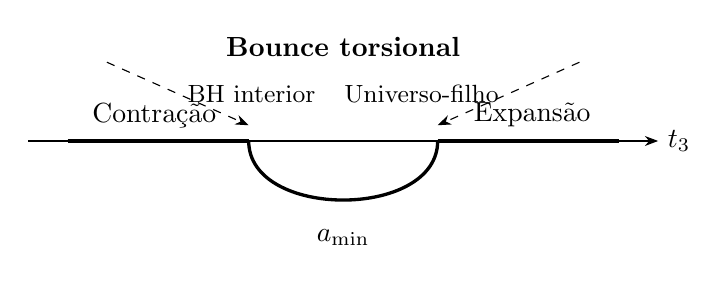
\begin{tikzpicture}[>=Stealth]
  % timeline
  \draw[->] (-4,0)--(4,0) node[right]{$t_{3}$};
  % contraction
  \draw[very thick] (-3.5,0) -- (-1.2,0);
  \node[above] at (-2.4,0.05){Contração};
  % minimum radius
  \draw[very thick] (-1.2,0).. controls +(0,-1) and +(0,-1) .. (1.2,0);
  \node[below] at (0,-1){$a_{\min}$};
  % expansion
  \draw[very thick] (1.2,0) -- (3.5,0);
  \node[above] at (2.4,0.05){Expansão};
  % BH arrow
  \draw[->,dashed] (-3,1) -- (-1.2,0.2) node[midway,right]{{\small BH interior}};
  \draw[->,dashed] (3,1) -- (1.2,0.2) node[midway,left]{{\small Universo-filho}};
  \node at (0,1.2){\textbf{Bounce torsional}};
 \end{tikzpicture}
 \caption{Sequência simplificada do bounce torsional: contração do universo--pai entra no interior do buraco negro, atinge raio mínimo $a_{\min}$ devido à torção e expande como universo--filho.}
 \label{fig:bounce}
\end{figure}

\subsection{Condição Schwarzschild do universo}
Para $M_{U}=6\times10^{53}$ kg e $R_{\text{obs}}=4.4\times10^{26}$ m, $2GM_{U}/c^{2}R_{\text{obs}}=0.98$ (Eq.~\eqref{eq:schw}).

%-------------------------------------------------------
\section{Rotação Global e Herança de Estrutura}\label{sec:rotation}
Momento angular herdado $\lambda\equiv Jc/GM^{2}\approx10^{-3}$ gera excesso de quiralidade observado em JWST.

%------------------  Spin Figure ----------------------
\begin{figure}[h]
 \centering
 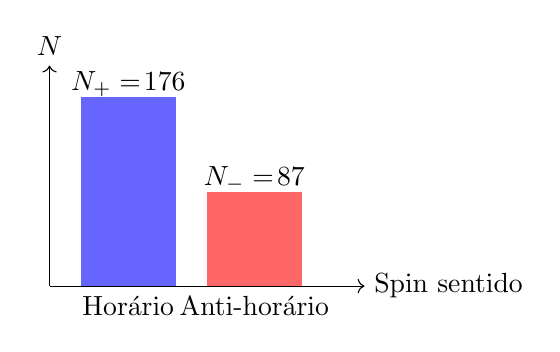
\begin{tikzpicture}[x=0.08cm,y=0.08cm]
  % histogram axes
  \draw[->] (0,0)--(50,0) node[right]{$\text{Spin sentido}$};
  \draw[->] (0,0)--(0,35) node[above]{$N$};
  % bars
  \fill[blue!60] (5,0) rectangle (20,30);
  \fill[red!60] (25,0) rectangle (40,15);
  \node[below] at (12.5,0){Horário};
  \node[below] at (32.5,0){Anti-horário};
  \node at (12.5,32){$N_{+}=\!176$};
  \node at (32.5,17){$N_{-}=\!87$};
 \end{tikzpicture}
 \caption{Distribuição qualitativa de rotações de galáxias no campo JADES (JWST). CTMCK prevê assimetria $N_{+}/N_{-}\approx2$.}
 \label{fig:spinJWST}
\end{figure}

%-------------------------------------------------------
\section{Early Massive Galaxies and JWST}\label{sec:jwst}
Perturbações herdadas ($\delta\rho/\rho\sim10^{-2}$) colapsam antes de $z\sim12$, compatíveis com discos massivos de $10^{11}M_{\odot}$ detectados.

%-------------------------------------------------------
\section{Energy--Dark as Temporal Gradient}\label{sec:darkenergy}
Curvatura diferencial $\Delta K_{t}$ gera $\rho_{\Lambda}=c^{4}\Delta K_{t}/8\pi G\approx5.9\times10^{-27}\,\text{kg m}^{-3}$.

%-------------------------------------------------------
\section{Observational Signatures}\label{sec:obs}
\begin{enumerate}
 \item \textbf{Preferred spin axis}: assimetria $>3\sigma$ prevista (Fig.~\ref{fig:spinJWST}).
 \item \textbf{Modified Hubble drift}: Fig.~\ref{fig:Hubble}.
 \item \textbf{Primordial torsional GW}: pico luminosa em $10^{-2}$ Hz.
\end{enumerate}

%------------------  Hubble Figure (unchanged) ---------
\begin{figure}[h]
 \centering
 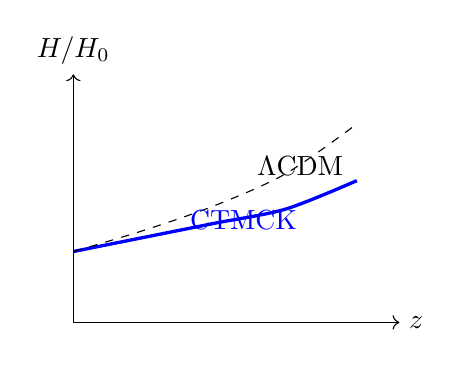
\begin{tikzpicture}[scale=0.9]
  \draw[->] (0,0)--(4.6,0) node[right]{$z$};
  \draw[->] (0,0)--(0,3.5) node[above]{$H/H_{0}$};
  \draw[very thick,blue] plot[smooth]coordinates{(0,1)(1,1.2)(2,1.4)(3,1.6)(4,2.0)};
  \draw[dashed] plot[smooth]coordinates{(0,1)(1,1.3)(2,1.65)(3,2.1)(4,2.8)};
  \node at (3.2,2.2){$\Lambda$CDM};
  \node[color=blue] at (2.4,1.45){CTMCK};
 \end{tikzpicture}
 \caption{Predicted reduced Hubble parameter in CTMCK versus $\Lambda$CDM. Numerical data in supplementary notebook.}
 \label{fig:Hubble}
\end{figure}

%-------------------------------------------------------
\section{Discussion}\label{sec:discussion}
Strengths, open issues (CMB B modes, BBN consistency), experimental roadmap.

%-------------------------------------------------------
\section{Conclusion}\label{sec:conclusion}
CTMCK bounce cosmology matches JWST anomalies, produces testable spin asymmetry and predicts a torsional GW background.

%-------------------   BIBLIOGRAPHY   -------------------
\bibliographystyle{unsrt}
\bibliography{ctmck_cosmo_refs}

\end{document}
